\documentclass[11pt,compress,t,notes=noshow, xcolor=table]{beamer}
\usepackage[]{graphicx}\usepackage[]{color}
% maxwidth is the original width if it is less than linewidth
% otherwise use linewidth (to make sure the graphics do not exceed the margin)
\makeatletter
\def\maxwidth{ %
  \ifdim\Gin@nat@width>\linewidth
    \linewidth
  \else
    \Gin@nat@width
  \fi
}
\makeatother

\newcommand{\citebutton}[2]{%
\beamergotobutton{\href{#2}{#1}}%
}

\newcommand{\blu}[1]{\textcolor{blue}{#1}}
\newcommand{\org}[1]{\textcolor{orange}{#1}}
\newcommand{\ques}{\textbf{\textcolor{red}{Question:  }}}
\newcommand{\questionssofar}{\begin{frame}\frametitle{Any questions?}\end{frame}}

\newcommand\warning{%
 \makebox[1.4em][c]{%
 \makebox[0pt][c]{\raisebox{.1em}{\scriptsize!}}%
 \makebox[0pt][c]{\color{red}\normalsize$\bigtriangleup$}}}%

\definecolor{fgcolor}{rgb}{0.345, 0.345, 0.345}
\newcommand{\hlnum}[1]{\textcolor[rgb]{0.686,0.059,0.569}{#1}}%
\newcommand{\hlstr}[1]{\textcolor[rgb]{0.192,0.494,0.8}{#1}}%
\newcommand{\hlcom}[1]{\textcolor[rgb]{0.678,0.584,0.686}{\textit{#1}}}%
\newcommand{\hlopt}[1]{\textcolor[rgb]{0,0,0}{#1}}%
\newcommand{\hlstd}[1]{\textcolor[rgb]{0.345,0.345,0.345}{#1}}%
\newcommand{\hlkwa}[1]{\textcolor[rgb]{0.161,0.373,0.58}{\textbf{#1}}}%
\newcommand{\hlkwb}[1]{\textcolor[rgb]{0.69,0.353,0.396}{#1}}%
\newcommand{\hlkwc}[1]{\textcolor[rgb]{0.333,0.667,0.333}{#1}}%
\newcommand{\hlkwd}[1]{\textcolor[rgb]{0.737,0.353,0.396}{\textbf{#1}}}%
\let\hlipl\hlkwb

\usepackage{framed}
\makeatletter
\newenvironment{kframe}{%
 \def\at@end@of@kframe{}%
 \ifinner\ifhmode%
  \def\at@end@of@kframe{\end{minipage}}%
  \begin{minipage}{\columnwidth}%
 \fi\fi%
 \def\FrameCommand##1{\hskip\@totalleftmargin \hskip-\fboxsep
 \colorbox{shadecolor}{##1}\hskip-\fboxsep
     % There is no \\@totalrightmargin, so:
     \hskip-\linewidth \hskip-\@totalleftmargin \hskip\columnwidth}%
 \MakeFramed {\advance\hsize-\width
   \@totalleftmargin\z@ \linewidth\hsize
   \@setminipage}}%
 {\par\unskip\endMakeFramed%
 \at@end@of@kframe}
\makeatother

\definecolor{shadecolor}{rgb}{.97, .97, .97}
\definecolor{messagecolor}{rgb}{0, 0, 0}
\definecolor{warningcolor}{rgb}{1, 0, 1}
\definecolor{errorcolor}{rgb}{1, 0, 0}
\newenvironment{knitrout}{}{} % an empty environment to be redefined in TeX

\usepackage{alltt}
\newcommand{\SweaveOpts}[1]{}  % do not interfere with LaTeX
\newcommand{\SweaveInput}[1]{} % because they are not real TeX commands
\newcommand{\Sexpr}[1]{}       % will only be parsed by R
\newcommand{\xmark}{\ding{55}}%


\usepackage[english]{babel}
\usepackage[utf8]{inputenc}

\usepackage{dsfont}
\usepackage{verbatim}
\usepackage{amsmath}
\usepackage{amsfonts}
\usepackage{amssymb}
\usepackage{bm}
\usepackage{csquotes}
\usepackage{multirow}
\usepackage{longtable}
\usepackage{booktabs}
\usepackage{enumerate}
\usepackage[absolute,overlay]{textpos}
\usepackage{psfrag}
\usepackage{algorithm}
\usepackage{algpseudocode}
\usepackage{eqnarray}
\usepackage{arydshln}
\usepackage{tabularx}
\usepackage{placeins}
\usepackage{tikz}
\usepackage{setspace}
\usepackage{colortbl}
\usepackage{mathtools}
\usepackage{wrapfig}
\usepackage{bm}
\usepackage{amsmath}
\usepackage{pifont}

\usetikzlibrary{shapes.multipart,shapes,arrows,automata,positioning,calc,chains,trees, shadows}
\tikzset{
  %Define standard arrow tip
  >=stealth',
  %Define style for boxes
  punkt/.style={
    rectangle,
    rounded corners,
    draw=black, very thick,
    text width=6.5em,
    minimum height=2em,
    text centered},
  % Define arrow style
  pil/.style={
    ->,
    thick,
    shorten <=2pt,
    shorten >=2pt,}
}

\tikzstyle{vec}=[draw, rectangle, fill = white, minimum width=5mm, minimum height=1cm, inner sep = 2pt]

\usepackage{subfig}

% Defines macros and environments
\usepackage{../../style/lmu-lecture}


\let\code=\texttt
\let\proglang=\textsf

\setkeys{Gin}{width=0.9\textwidth}

\setbeamertemplate{frametitle}{\expandafter\uppercase\expandafter\insertframetitle}

\usepackage{bbm}
% basic latex stuff
\newcommand{\pkg}[1]{{\fontseries{b}\selectfont #1}} %fontstyle for R packages
\newcommand{\lz}{\vspace{0.5cm}} %vertical space
\newcommand{\dlz}{\vspace{1cm}} %double vertical space
\newcommand{\oneliner}[1] % Oneliner for important statements
{\begin{block}{}\begin{center}\begin{Large}#1\end{Large}\end{center}\end{block}}


%new environments
\newenvironment{vbframe}  %frame with breaks and verbatim
{
 \begin{frame}[containsverbatim,allowframebreaks]
}
{
\end{frame}
}

\newenvironment{vframe}  %frame with verbatim without breaks (to avoid numbering one slided frames)
{
 \begin{frame}[containsverbatim]
}
{
\end{frame}
}

\newenvironment{blocki}[1]   % itemize block
{
 \begin{block}{#1}\begin{itemize}
}
{
\end{itemize}\end{block}
}

\newenvironment{fragileframe}[2]{  %fragile frame with framebreaks
\begin{frame}[allowframebreaks, fragile, environment = fragileframe]
\frametitle{#1}
#2}
{\end{frame}}


\newcommand{\myframe}[2]{  %short for frame with framebreaks
\begin{frame}[allowframebreaks]
\frametitle{#1}
#2
\end{frame}}

\newcommand{\remark}[1]{
  \textbf{Remark:} #1
}


\newenvironment{deleteframe}
{
\begingroup
\usebackgroundtemplate{
\includegraphics[width=\paperwidth,height=\paperheight]{../style/color/red.png}}
 \begin{frame}
}
{
\end{frame}
\endgroup
}
\newenvironment{simplifyframe}
{
\begingroup
\usebackgroundtemplate{
\includegraphics[width=\paperwidth,height=\paperheight]{../style/color/yellow.png}}
 \begin{frame}
}
{
\end{frame}
\endgroup
}\newenvironment{draftframe}
{
\begingroup
\usebackgroundtemplate{
\includegraphics[width=\paperwidth,height=\paperheight]{../style/color/green.jpg}}
 \begin{frame}
}
{
\end{frame}
\endgroup
}
% https://tex.stackexchange.com/a/261480: textcolor that works in mathmode
\makeatletter
\renewcommand*{\@textcolor}[3]{%
  \protect\leavevmode
  \begingroup
    \color#1{#2}#3%
  \endgroup
}
\makeatother





\input{../../latex-math/basic-math.tex}
\input{../../latex-math/basic-ml.tex}
\newcommand*\POS[1]{\textsubscript{\texttt{#1}}} % tag with part of speech
\usepackage{qtree} %parse tree

\newcommand{\titlefigure}{figure/bengio03.png}
\newcommand{\learninggoals}{
\item grasp importance of the ``look-up table`` a.k.a. embedding layer
\item understand computational implications of language modeling}

\title{Basics}
% \author{}
\institute{\href{https://slds-lmu.github.io/lecture_dl4nlp/}{slds-lmu.github.io/lecture\_dl4nlp}}
\date{}

\begin{document}
\lecturechapter{Neural Probabilistic Language Model}
\lecture{Deep Learning for NLP} % stays constant


% ------------------------------------------------------------------------------

\begin{frame}{What is a language model?}
\vspace{.5cm}
\begin{block}{Wikipedia says:}
    \begin{center}
    "A statistical language model is a probability distribution over sequences of words"
    \end{center}
\end{block}
\begin{block}{This means (a) assigning a probability to a sequence of words, e.g.}
    \[
    P(\mbox{\it "we are all interested in NLP"})
    \]
\end{block}
\begin{block}{and (b) assigning a probability to the likelihood of a word given a sequence of words, e.g.}
    \[
    P(\mbox{\it "NLP"} | \mbox{\it "we are all interested in"})
    \]
\end{block}
\end{frame}

% ------------------------------------------------------------------------------

\begin{vbframe}{cf. previous chapter}
	
\vfill

\textbf{Predict the next token:}

\begin{figure}
	\centering
		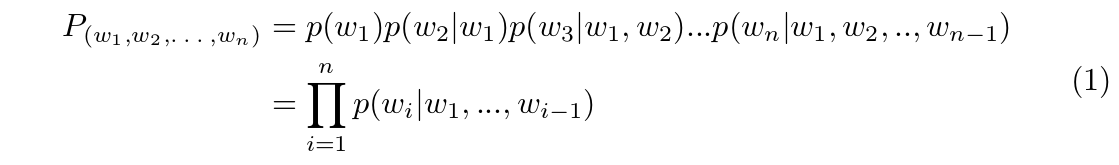
\includegraphics[width = 11cm]{figure/language-modeling.png}\\ 
		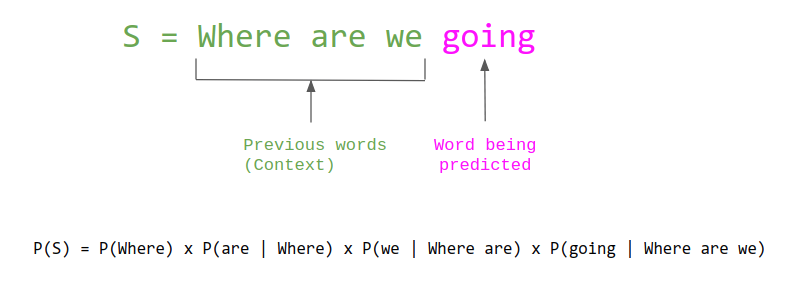
\includegraphics[width = 11cm]{figure/language-modeling2.png}\\
	\beamergotobutton{\href{https://thegradient.pub/understanding-evaluation-metrics-for-language-models/}{Source: The Gradient}}
\end{figure}

\vfill

\end{vbframe}

% ------------------------------------------------------------------------------

\begin{frame}{Making use of the Markov-Assumption}

\vfill

\begin{block}{The Markov-Assumption}
    \begin{itemize}
        \item "The future is independent of the past given the present"
        \item In NLP context:\\
        $\rightarrow$ Next word only depends on the $k$ previous words\\
        $\rightarrow$ $k$th order markov assumption with k to be chosen manually
    \end{itemize}
\end{block}
\begin{block}{"Traditional" count-based models}
    \begin{itemize}
        \item Good baselines, but severe shortcomings
        \item Lacking the ability to generalize
    \end{itemize}
\end{block}

\vfill

\end{frame}

% ------------------------------------------------------------------------------

\begin{frame}{What are potential problems?}

\vfill

\begin{block}{Curse of dimensionality}
    \begin{itemize}
        \item Linear increase in context size leads to an exponential increase in the number of parameters
        \item Considering a vocabulary of size $|V| = 100,000$:\\
        $\rightarrow$ Already for bi-grams: $|V|^2 = 10^{10}$ possible combinations
    \end{itemize}
\end{block}
\begin{block}{Sparsity}
    \begin{itemize}
        \item Again, considering $|V| = 1.000.000$ \& bi-grams as context
        \item Unlikely to observe all of them bi-gram combinations
        \begin{enumerate}[(a)]
            \item ever
            \item often
        \end{enumerate}
    \end{itemize}
\end{block}

\vfill

\end{frame}

% ------------------------------------------------------------------------------

\begin{frame}{A Neural Probabilistic Language Model}

\vfill

\begin{block}{Idea}
        \begin{itemize}
        \item Using a neural network induces non-linearity and overcomes the shortcomings of traditional models
        \begin{enumerate}[(a)]
            \item Linear increase in $\#$parameters with increasing context size
            \item Better generalization
        \end{enumerate}
        \item \textbf{Input:} {\it Context of $(n-1)$ words} \hfill $[w_{(t-n+1):(t-1)}]$
        \item \textbf{In between:} 
        \begin{itemize}
            \item {\it Look-up table} \hfill $[\vec w^{({w_{t-n+1}})}; .. ; \vec w^{({w_{t-2}})}; \vec w^{({w_{t-1}})}]$
            \item[]
            \item {\it Non-linearity} \hfill e.g. tanh, ReLU
        \end{itemize}
        \item \textbf{Output:}\\{\it Probability distribution over the next word} \hfill $P(w_t|w_{(t-n+1):(t-1)})$
        \end{itemize}
\end{block}

\vfill

\end{frame}

% ------------------------------------------------------------------------------

\begin{frame}{Graphical illustration}

\vfill

\begin{figure}
    \centering
    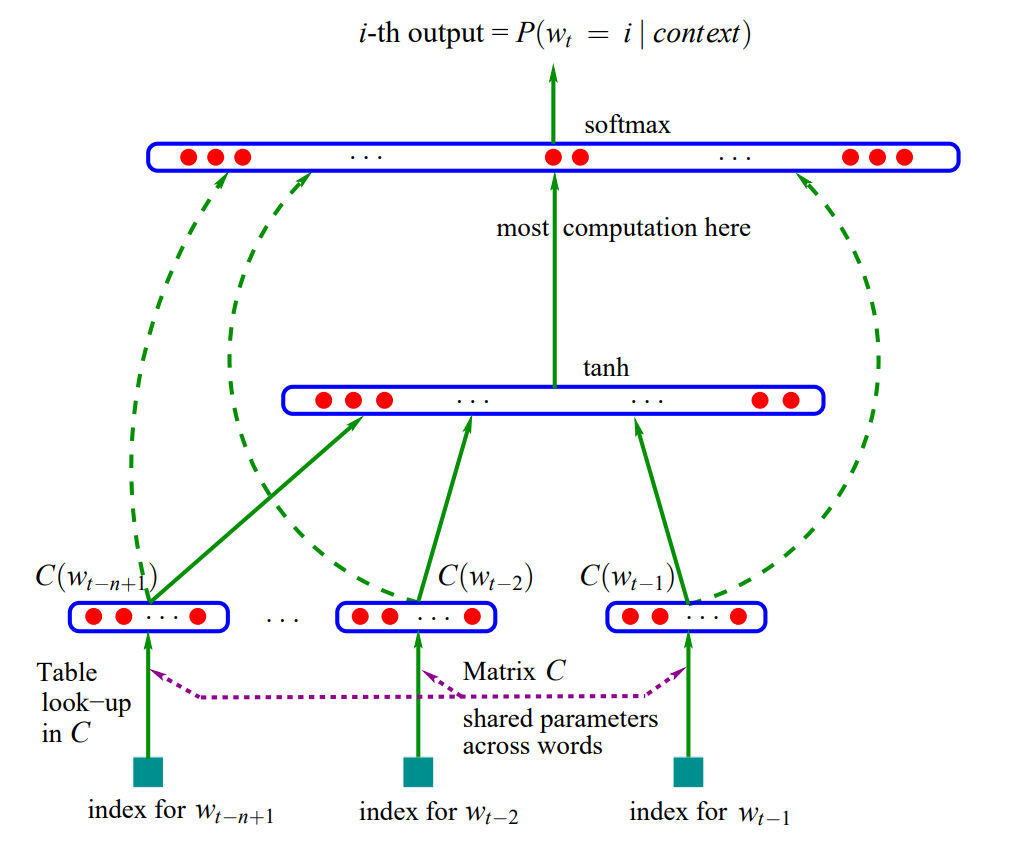
\includegraphics[width=8cm]{figure/bengio03.png}\\
		\beamergotobutton{\href{https://www.jmlr.org/papers/volume3/bengio03a/bengio03a.pdf}{Source: Bengio et al., 2003}}
\end{figure}

\scriptsize{\textit{Note: C($\cdot$) replaced by $\vec w^{(\cdot)}$ on the previous slide.}}

\vfill

\end{frame}

% ------------------------------------------------------------------------------

\begin{frame}{What could be problematic?}

\vfill

\begin{block}{Computational cost}
    \begin{itemize}
        \item Vanilla softmax is expensive
        \item Proposed solution(s): 
        \begin{enumerate}
            \item Hierarchical softmax \beamergotobutton{\href{https://www.iro.umontreal.ca/~lisa/pointeurs/hierarchical-nnlm-aistats05.pdf}{Morin and Bengio, 2005}}
            \item Sampling Approaches (next chapter)
        \end{enumerate}
    \end{itemize}
\end{block}
\begin{block}{Still relying on the markov assumption}
    \begin{itemize}
        \item Context window has to be specified manually
    \end{itemize}
\end{block}

\vfill

\end{frame}

% ------------------------------------------------------------------------------

\endlecture
\end{document}
